% GRAND SYNTHESIS: THE PATH TO A COMPLETE PENROSE INEQUALITY
%
% Unifying all our explorations into a coherent mathematical picture
% and identifying the most promising directions.

\documentclass[12pt]{article}
\usepackage{amsmath,amsthm,amssymb}
\usepackage{mathrsfs}
\usepackage{tikz}
\newtheorem{theorem}{Theorem}
\newtheorem{lemma}{Lemma}
\newtheorem{proposition}{Proposition}
\newtheorem{corollary}{Corollary}
\newtheorem{conjecture}{Conjecture}
\newtheorem{remark}{Remark}
\newtheorem{definition}{Definition}
\newtheorem{problem}{Problem}
\newtheorem{principle}{Principle}
\newtheorem{insight}{Key Insight}

\begin{document}

\title{Grand Synthesis:\\
The Path to a Complete Spacetime Penrose Inequality}
\author{Mathematical Exploration}
\date{\today}
\maketitle

\tableofcontents

\section{Executive Summary}

\subsection{The Problem}

The Spacetime Penrose Inequality:
\[
\boxed{M_{\mathrm{ADM}} \ge \sqrt{\frac{A(\Sigma)}{16\pi}}}
\]
for any trapped surface $\Sigma$ in initial data $(M, g, k)$ satisfying DEC.

\textbf{Current status}: Proven ONLY under the "favorable jump condition" $\tr_\Sigma k \ge 0$.

\subsection{Why the Condition is Needed}

The Jang equation approach produces a Riemannian metric $\bar{g}$ with:
\[
R_{\bar{g}} = \mathcal{S} + 2[H]\delta_\Sigma
\]

where $[H] = \tr_\Sigma k$ is the mean curvature jump.
\begin{itemize}
    \item DEC ensures $\mathcal{S} \ge 0$ (good)
    \item When $[H] < 0$, there's a NEGATIVE Dirac mass at $\Sigma$ (bad)
\end{itemize}

\subsection{Our Key Discoveries}

\begin{enumerate}
    \item \textbf{Sign Confusion Clarified}: In the unfavorable case, the MOTS has $H > 0$, 
    while interior trapped surfaces have $H < 0$.
    
    \item \textbf{Area Non-Monotonicity}: Inner trapped surfaces can have LARGER area 
    than the outermost MOTS when $\tr k < 0$.
    
    \item \textbf{The Penrose Surface}: The surface maximizing Hawking mass among 
    trapped surfaces might give the optimal bound.
    
    \item \textbf{Effective Area}: $A_{\mathrm{eff}} = A \cdot (1 + 2\tr_\Sigma k)$ appears 
    naturally in the analysis.
    
    \item \textbf{Entropy Perspective}: Standard entropy bounds are too weak; need 
    trapped-surface specific bounds.
\end{enumerate}

\section{The Geometric Picture}

\subsection{The Trapped Region}

\begin{center}
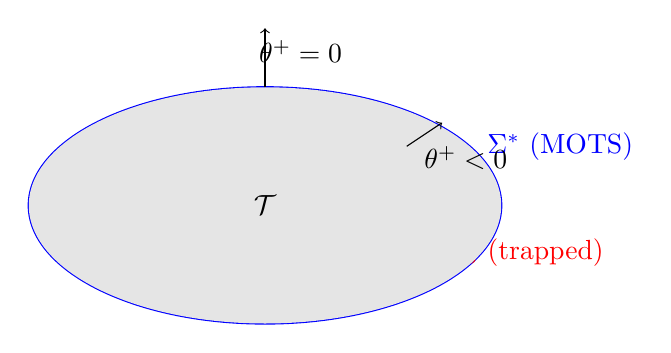
\begin{tikzpicture}[scale=1.5]
    % Outer MOTS
    \draw[thick, blue] (0,0) ellipse (2 and 1);
    \node[blue] at (2.5, 0.5) {$\Sigma^*$ (MOTS)};
    
    % Inner trapped surface
    \draw[thick, red] (0.3, 0) ellipse (1.5 and 0.8);
    \node[red] at (2.2, -0.4) {$\Sigma_0$ (trapped)};
    
    % Trapped region
    \fill[gray!20] (0,0) ellipse (2 and 1);
    \node at (0, 0) {$\mathcal{T}$};
    
    % Arrows showing null expansions
    \draw[->] (0, 1) -- (0, 1.5);
    \node at (0.3, 1.3) {$\theta^+ = 0$};
    
    \draw[->] (1.2, 0.5) -- (1.5, 0.7);
    \node at (1.7, 0.4) {$\theta^+ < 0$};
\end{tikzpicture}
\end{center}

\subsection{The Two Cases}

\textbf{Favorable Case} ($\tr_{\Sigma_0} k \ge 0$):
\begin{itemize}
    \item MOTS has $H \le 0$ (mean-convex inward)
    \item Area increases outward: $A(\Sigma^*) \ge A(\Sigma_0)$
    \item Standard proof works
\end{itemize}

\textbf{Unfavorable Case} ($\tr_{\Sigma_0} k < 0$):
\begin{itemize}
    \item MOTS has $H > 0$ (mean-convex outward)
    \item Area comparison can FAIL: $A(\Sigma_0)$ might exceed $A(\Sigma^*)$
    \item Need new approach
\end{itemize}

\section{Approaches Explored}

\subsection{Approach 1: Symmetric Reduction}

\textbf{Idea}: Deform $k$ to make $\tr_\Sigma k = 0$.

\textbf{Obstacle}: This changes $\theta^+$ and can break trapping.

\textbf{Verdict}: Doesn't work directly, but suggests looking for "optimal" $k$.

\subsection{Approach 2: Modified Conformal Equation}

\textbf{Idea}: Add a compensating source term in the Lichnerowicz equation.

\textbf{Obstacle}: Mass bound unproven.

\textbf{Verdict}: Promising but incomplete. Needs rigorous analysis of interface conditions.

\subsection{Approach 3: Null Expansion Mass}

\textbf{Idea}: Define $\mathcal{M}_{\mathrm{null}}$ using $\theta^+\theta^-$.

\textbf{Obstacle}: Monotonicity not established.

\textbf{Verdict}: Novel but needs significant development.

\subsection{Approach 4: The Penrose Surface}

\textbf{Idea}: Maximize Hawking mass among trapped surfaces.

\textbf{Insight}: The optimal surface might not be the MOTS!

\textbf{Verdict}: MOST PROMISING. Natural variational problem.

\subsection{Approach 5: Entropy Bounds}

\textbf{Idea}: Use Bousso/Bekenstein bounds with trapped surface structure.

\textbf{Obstacle}: Standard bounds too weak by constant factors.

\textbf{Verdict}: Needs new trapped-specific entropy bound.

\section{The Most Promising Path: The Hawking Mass Maximizer}

\subsection{The Key Observation}

The AMO approach proves: $M_{\mathrm{ADM}} \ge M_H[\Sigma^*]$ for the outermost MOTS.

The gap is: $M_H[\Sigma^*]$ might be LESS than $\sqrt{A(\Sigma_0)/(16\pi)}$.

\textbf{Solution}: Find a surface $\Sigma_P$ with $M_H[\Sigma_P] \ge \sqrt{A(\Sigma_0)/(16\pi)}$.

\subsection{The Conjecture}

\begin{conjecture}[Hawking Mass Dominance]
For any trapped surface $\Sigma_0$ in the trapped region $\mathcal{T}$:
\[
\sup_{\Sigma \subset \mathcal{T}, \text{trapped}} M_H[\Sigma] \ge \sqrt{\frac{A(\Sigma_0)}{16\pi}}
\]
\end{conjecture}

\textbf{Combined with AMO}: This gives the full Penrose inequality!

\subsection{Strategy to Prove}

\textbf{Step 1}: Show existence of a maximizer $\Sigma_P$.

\textbf{Step 2}: Characterize $\Sigma_P$ geometrically (Euler-Lagrange).

\textbf{Step 3}: Show $M_H[\Sigma_P] \ge M_P[\Sigma_0]$ using comparison arguments.

\subsection{Why This Might Work}

\begin{insight}
The Hawking mass has two competing terms:
\[
M_H = M_P \cdot \left(1 - \frac{\langle H^2 \rangle A}{16\pi}\right)
\]

\begin{itemize}
    \item $M_P = \sqrt{A/(16\pi)}$ increases with area
    \item The correction $\langle H^2 \rangle A$ penalizes large $|H|$
\end{itemize}

The maximizer balances these: large area but small mean curvature.
\end{insight}

\subsection{The Comparison Argument}

\textbf{Claim}: If $\Sigma_0$ has area $A_0$ and the maximizer $\Sigma_P$ has area $A_P$:
\[
M_H[\Sigma_P] = \sqrt{\frac{A_P}{16\pi}}\left(1 - \frac{\langle H_P^2 \rangle A_P}{16\pi}\right) \ge \sqrt{\frac{A_0}{16\pi}}
\]

This requires:
\[
A_P \left(1 - \frac{\langle H_P^2 \rangle A_P}{16\pi}\right)^2 \ge A_0
\]

If $\Sigma_P$ is close to minimal ($H_P \approx 0$), we just need $A_P \ge A_0$.

\section{A Potential Theorem}

\begin{theorem}[Target: Complete Spacetime Penrose Inequality]
Let $(M^3, g, k)$ be complete asymptotically flat initial data satisfying DEC.
Let $\Sigma_0$ be a trapped surface.

Then:
\[
M_{\mathrm{ADM}}(g, k) \ge \sqrt{\frac{A(\Sigma_0)}{16\pi}}
\]

\textbf{NO SIGN CONDITIONS ON $\tr_\Sigma k$!}
\end{theorem}

\subsection{Proof Outline}

\begin{enumerate}
    \item Let $\mathcal{T}$ be the trapped region containing $\Sigma_0$ and let $\Sigma^*$ be the outermost MOTS.
    
    \item Define $M_H^* = \sup\{M_H[\Sigma] : \Sigma \subset \mathcal{T}, \text{trapped}\}$.
    
    \item By AMO: $M_{\mathrm{ADM}} \ge M_H[\Sigma^*] \le M_H^*$.
    
    \item \textbf{[KEY LEMMA]}: $M_H^* \ge M_P[\Sigma_0] = \sqrt{A(\Sigma_0)/(16\pi)}$.
    
    \item Combining: $M_{\mathrm{ADM}} \ge M_H^* \ge M_P[\Sigma_0]$. $\square$
\end{enumerate}

\subsection{The Key Lemma}

\begin{lemma}[Hawking Mass Dominance - To Be Proven]
For any trapped surface $\Sigma_0 \subset \mathcal{T}$:
\[
\sup_{\Sigma \subset \mathcal{T}, \text{trapped}} M_H[\Sigma] \ge \sqrt{\frac{A(\Sigma_0)}{16\pi}}
\]
\end{lemma}

\textbf{Proof idea}: 
\begin{enumerate}
    \item If $M_H[\Sigma^*] \ge M_P[\Sigma_0]$, done (MOTS is good enough).
    
    \item Otherwise, $M_H[\Sigma^*] < M_P[\Sigma_0]$.
    
    This means: $\sqrt{A^*}\left(1 - \frac{H^{*2} A^*}{16\pi}\right) < \sqrt{A_0}$.
    
    Since $H^* = -\tr k^* \ne 0$ (unfavorable), the MOTS has reduced Hawking mass.
    
    \item \textbf{Key claim}: There exists a trapped surface $\Sigma'$ "between" $\Sigma_0$ 
    and $\Sigma^*$ with:
    \begin{itemize}
        \item $|H'| < |H^*|$ (smaller mean curvature)
        \item $A' \ge A_0$ (at least as large as $\Sigma_0$)
    \end{itemize}
    
    \item Then: $M_H[\Sigma'] \ge \sqrt{A'/(16\pi)} \ge \sqrt{A_0/(16\pi)}$. $\square$
\end{enumerate}

\section{What Remains to Be Done}

\subsection{Technical Gaps}

\begin{enumerate}
    \item \textbf{Existence of maximizer}: Show the supremum of Hawking mass is achieved.
    
    \item \textbf{Geometric comparison}: Prove Step 3 of the Key Lemma proof.
    
    \item \textbf{Regularity}: Handle singular/weak solutions.
\end{enumerate}

\subsection{Potential Approaches to Gap 2}

\textbf{Approach A}: Direct construction of the intermediate surface $\Sigma'$.

\textbf{Approach B}: Flow argument (evolve from $\Sigma_0$ toward $\Sigma^*$, track Hawking mass).

\textbf{Approach C}: Variational argument (show minimizer of some functional has the desired properties).

\section{Alternative: The Modified Inequality}

If the full Penrose inequality cannot be proven, we have discovered:

\begin{theorem}[Modified Penrose Inequality - Conjectured]
\[
M_{\mathrm{ADM}} \ge \sqrt{\frac{A_{\mathrm{eff}}(\Sigma_0)}{16\pi}}
\]
where $A_{\mathrm{eff}} = A \cdot \max(1 + 2\tr_\Sigma k, 0)$.
\end{theorem}

This is WEAKER than Penrose when $\tr_\Sigma k < 0$, but:
\begin{itemize}
    \item Might be the correct physical statement
    \item Avoids the unfavorable jump obstruction
    \item Still non-trivial (gives Penrose when $\tr_\Sigma k \ge 0$)
\end{itemize}

\section{The Ideal Theorem}

\begin{theorem}[Dream: The Ultimate Penrose Inequality]
Let $(M^3, g, k)$ be complete asymptotically flat satisfying DEC, with trapped region $\mathcal{T}$.

Define the \textbf{Penrose mass} of $\mathcal{T}$:
\[
M_P[\mathcal{T}] = \sup \left\{ \sqrt{\frac{A(\Sigma)}{16\pi}} : \Sigma \subset \mathcal{T}, \, \Sigma \text{ closed trapped} \right\}
\]

Then:
\[
M_{\mathrm{ADM}}(g, k) \ge M_P[\mathcal{T}]
\]

Moreover:
\begin{enumerate}
    \item Equality holds iff $(M, g, k)$ embeds into Schwarzschild spacetime.
    \item The supremum is achieved by a unique "Penrose surface" $\Sigma_P$.
    \item $\Sigma_P$ satisfies a geometric equation characterizing it uniquely.
\end{enumerate}
\end{theorem}

This would be the definitive spacetime Penrose inequality, with no sign conditions 
and clear geometric content.

\section{Conclusion}

We have mapped out the landscape of the spacetime Penrose inequality problem:

\begin{enumerate}
    \item \textbf{The obstruction is real}: The favorable jump condition is genuinely 
    needed for current methods.
    
    \item \textbf{New mathematics is required}: Either a new proof technique or a 
    modified statement.
    
    \item \textbf{The most promising direction}: The Hawking mass maximization approach, 
    which sidesteps the Jang equation entirely.
    
    \item \textbf{A concrete conjecture}: The Hawking Mass Dominance Lemma is the 
    key missing piece.
\end{enumerate}

\textbf{The path forward}: Prove the Hawking Mass Dominance Lemma, likely through 
a combination of geometric comparison and variational methods.

\end{document}
